\documentclass{article}
\PassOptionsToPackage{numbers,compress,sort}{natbib}
\usepackage[final]{neurips_2026}

\usepackage{booktabs}            % professional-quality tables
\usepackage{multirow}            % tabular cells spanning multiple rows
\usepackage{amsfonts}            % blackboard math symbols
\usepackage{amsmath, amssymb, amsthm, mathtools}
\usepackage{graphicx}            % figures
\usepackage{url}
\usepackage{microtype}

\newtheorem{definition}{Definition}
\newtheorem{proposition}[definition]{Proposition}
\newtheorem{remark}[definition]{Remark}

\title{A-Block: Clifford Neural Score Matching for Multi-Well Conformational Dynamics and Active Particle Sampling}

\author{%
  Erick Oduniyi\\
  Massachusetts Institute of Technology\\
  Cambridge, MA\\
  \texttt{erick000@media.mit.edu}\\
}

\setlength{\textfloatsep}{6pt plus 1pt minus 1pt}
\setlength{\floatsep}{5pt plus 1pt minus 1pt}
\setlength{\intextsep}{5pt plus 1pt minus 1pt}

\begin{document}

\maketitle

\begin{abstract}
Sampling multi-well free energy surfaces and navigating metastable conformational transition states are central challenges in molecular machine learning. Standard score-guided Langevin samplers and diffusion models operate over unconstrained Euclidean gradients, frequently suffering from kinetic trapping in deep potential wells. In this work, we present \textit{A-Block}: a Clifford Neural Score Matching framework that unifies 2D Geometric Algebra ($\operatorname{Cl}(2,0)$), non-reversible score-based stochastic differential equations, and active matter Langevin hydrodynamics. We parameterize continuous potential fields via a neural network trained through Denoising Score Matching (DSM), augmented with coordinate-free multivector rotor-dilator dynamics $(\sigma_i I - \kappa_i) \nabla V_\theta(\mathbf{x}_i)$. We characterize the Fokker--Planck stationarity conditions separating measure-preserving non-reversible Boltzmann sampling from non-equilibrium active confinement, and evaluate A-Block on a canonical three-basin landscape (Basins A, B, C) against unconditional Brownian dynamics, standard Langevin score matching, matched-contraction dilation ($\sigma=0$), and rotor-only dynamics ($\kappa = 0$). Across multi-seed evaluations, A-Block achieves the lowest Free Energy Surface reconstruction error ($\text{RMSE} = 1.059 \pm 0.031 \text{ kcal/mol}$ vs.\ $1.476 \pm 0.069 \text{ kcal/mol}$ for standard Langevin) and the highest inter-basin transition frequency ($22.48 \pm 0.15$ transitions/particle, $+62.2\%$ over matched dilation alone) while maintaining linear $O(N)$ per-step scaling. We further demonstrate programmable spatial particulate control across non-convex geometric attractors, establishing a preliminary geometric foundation for dihedral conformation sampling and active matter design.
\end{abstract}

\section{Introduction}

Characterizing complex free-energy landscapes, predicting metastable transition paths, and generating diverse biomolecular conformations are central objectives of molecular machine learning~\citep{noe2019boltzmann, hoogeboom2022equivariant, du2022molgen}. While score-based generative modeling and geometric deep learning have enabled rapid structural synthesis~\citep{bronstein2021geometric, song2020score}, sampling from rugged multi-well distributions remains computationally challenging. In physical systems with high free-energy barriers between metastable states—such as multi-state signaling proteins undergoing conformational interchange~\citep{devore2016single}—reversible overdamped Langevin samplers frequently suffer from kinetic trapping or poor saddle-region resolution.

Concurrently, mathematical analyses of non-reversible diffusions~\citep{hwang2005accelerating, lelievre2013optimal, duncan2016variance} and physical active matter hydrodynamics~\citep{marchetti2013, muller1979location} demonstrate that introducing divergence-free transverse circulation orthogonal to the potential gradient accelerates ergodic mixing and barrier crossing. Integrating non-reversible rotor dynamics with score-based neural fields presents a natural synergy: transverse circulation along score isolines drives trajectories laterally toward low-energy saddle points without degrading the learned potential surface.

In this paper, we introduce \textbf{A-Block} (Algebraic Block), a Clifford Neural Score Matching framework for multi-well conformational dynamics and spatial particulate control (Figure~\ref{fig:kinetic_trap_benchmark}). Rather than viewing kinetic trapping solely as a failure mode, we frame it as a physical phenomenon to be governed via two operating regimes: in \textit{equilibrium conformational sampling}, the multivector rotor ($\sigma I$) circulates trajectories along equipotential contours toward transition saddles while the dilator ($-\kappa$) maintains basin confinement; in \textit{non-equilibrium active matter control}, heightened contraction and chiral circulation drive ensembles into sharp non-convex geometric attractors. Our contributions are threefold: (1)~\textbf{Clifford Neural Score Architecture \& Fokker--Planck Analysis:} We couple a DSM-trained neural potential $V_\theta(\mathbf{x})$ with a $\operatorname{Cl}(2,0)$ rotor-dilator operator $(\sigma I - \kappa)\nabla V_\theta(\mathbf{x})$, establishing the exact Fokker--Planck conditions for Boltzmann stationarity vs.\ non-equilibrium steady-state confinement; (2)~\textbf{Decoupled Point-Measure \& Dihedral Scaling:} We show that replacing pairwise interaction graphs ($O(N^2)$) with empirical point measures $\mu_t$ yields $O(N)$ per-step complexity, while direct-sum planar rotors $\bigoplus_{k=1}^K \operatorname{Cl}(2,0)$ scale linearly as $4K$ rather than $2^{2K}$; and (3)~\textbf{Multi-Seed Empirical Grounding \& Component Ablations:} Across multi-seed benchmarks, matched-contraction ablations ($\sigma=0, \kappa$), and timestep/binning sensitivity checks, we demonstrate that A-Block achieves both the lowest Free Energy Surface (FES) RMSE and the highest inter-basin transition rate.\footnote{Public code, trained weights, and reproducibility tutorials: \url{https://github.com/eoduniyi/ablock}}

\section{The A-Block Architecture: Clifford Neural Score Matching}

An \textit{A-Block} models a modular ensemble of $N$ particulate states $\mathbf{x}_i \in \Omega \subset \mathbb{R}^2$ evolving inside a bounded virtual aperture (a continuous ``Petri dish'') under a learned neural score field. Physically, the potential $V(\mathbf{x})$ carved into this aperture can represent either a discrete multi-well conformational surface (Basins A, B, C in Figure~\ref{fig:kinetic_trap_benchmark}, modeling a $(\phi, \psi)$ dihedral pair) or a continuous non-convex morphological trench (the letterform attractors in Appendix~\ref{sec:appendix}).

\subsection{Neural Potential Parameterization, Energy Calibration, and DSM Training}

Let $\mathbf{x} \in \mathbb{R}^2$ denote internal reaction coordinates governed by a multi-well potential $V(\mathbf{x})$ (in $\text{kcal/mol}$) at thermal energy $k_B T = 0.6\text{ kcal/mol}$. We model the target Boltzmann density $p(\mathbf{x}) \propto \exp(-V(\mathbf{x}) / k_B T)$ via a neural network (\texttt{CliffordScoreNet}) parameterizing a scalar potential $V_\theta(\mathbf{x}): \mathbb{R}^2 \to \mathbb{R}$ alongside rotor-dilator control channels $(\sigma(\mathbf{x}), \kappa(\mathbf{x}))$.

\textbf{Network Architecture and Training Protocol.} \texttt{CliffordScoreNet} is a 4-layer multilayer perceptron ($\mathbb{R}^2 \to 64 \to 64 \to 64 \to \mathbb{R}^3$) with $\operatorname{SiLU}$ activations. To generate an unlabeled equilibrium training corpus without ground-truth force supervision, we draw $12{,}000$ coordinates ($4{,}000$ initialized per basin with Gaussian dispersion $0.35\text{--}0.40$) and apply $150$ thermal relaxation steps ($dt = 0.012, k_B T = 0.6$). The network is trained for $250$ epochs via Vincent--Song Denoising Score Matching (DSM)~\citep{song2020score} using $\operatorname{AdamW}$ ($\text{lr} = 2 \times 10^{-3}$, weight decay $10^{-5}$, cosine annealing, gradient clipping at $1.0$) over multi-scale noise perturbations $\sigma_n \in \{0.05, 0.10, 0.20\}$:
\vspace{-1mm}
\begin{equation}
\mathcal{L}_{\text{DSM}}(\theta) = \mathbb{E}_{\mathbf{x} \sim p_{\text{data}},\, \sigma_n,\, \boldsymbol{\epsilon} \sim \mathcal{N}(0, \mathbf{I})}\Bigl[ \sigma_n^2 \bigl\| -\nabla_{\mathbf{\tilde{x}}} V_\theta(\mathbf{\tilde{x}}) - \nabla_{\mathbf{\tilde{x}}} \log q_{\sigma_n}(\mathbf{\tilde{x}}|\mathbf{x}) \bigr\|^2 \Bigr],
\label{eq:score_matching}
\end{equation}
\vspace{-1mm}
where $\mathbf{\tilde{x}} = \mathbf{x} + \sigma_n \boldsymbol{\epsilon}$ and $\nabla_{\mathbf{\tilde{x}}} \log q_{\sigma_n}(\mathbf{\tilde{x}}|\mathbf{x}) = -\boldsymbol{\epsilon}/\sigma_n$. Because DSM regressing against $-\boldsymbol{\epsilon}/\sigma_n^2$ estimates the dimensionless score $\nabla_{\mathbf{x}} \log p(\mathbf{x}) = -\nabla V(\mathbf{x}) / (k_B T)$, the learned potential satisfies $\nabla V_\theta(\mathbf{x}) \approx \alpha_E \nabla V(\mathbf{x})$ with empirical inverse-temperature scale factor $\alpha_E \approx (k_B T)^{-1} \approx 1.67\text{ (kcal/mol)}^{-1}$ (verified on our benchmark where $V_\theta$ spans $5.02$ dimensionless units across the $2.99\text{ kcal/mol}$ ground-truth basin span, yielding $\alpha_E = 1.678$).

\subsection{Geometric Algebra Formulation of Rotor-Dilator Dynamics ($\operatorname{Cl}(2,0)$)}

Standard score-guided Langevin dynamics evolve strictly along $-\nabla V_\theta(\mathbf{x})$. To introduce non-reversible circulation along equipotential contours, we work in the 2D Clifford Geometric Algebra $\operatorname{Cl}(2,0)$ with orthonormal basis $\{e_1, e_2\}$ and unit bivector pseudoscalar $I = e_1 e_2$ ($I^2 = -1$). While a monolithic $D$-dimensional Clifford algebra $\operatorname{Cl}(D,0)$ incurs $2^D$ basis growth, macromolecular backbones with $K$ dihedral hinges $(\phi_k, \psi_k)$ decompose into a direct sum of planar subalgebras $\bigoplus_{k=1}^K \operatorname{Cl}(2,0)$, scaling linearly as $4K$ rather than $2^{2K}$.

We define the multivector drift operator as a coupled \textit{rotor-dilator}:
\vspace{-1mm}
\begin{equation}
\mathbf{f}_i(\mathbf{x}_i) = (\sigma_i I - \kappa_i) \nabla V_\theta(\mathbf{x}_i),
\label{eq:clifford_flow}
\end{equation}
\vspace{-1mm}
where $I \nabla V_\theta = (-\partial_{y} V_\theta, \partial_{x} V_\theta)^\top$ rotates the gradient by $90^\circ$ to generate symplectic contour flow, $\sigma_i = 1.5 \tanh(\cdot) \in [-1.5, 1.5]$ controls rotor chirality, and $\kappa_i = \operatorname{softplus}(\cdot) + 0.1 \in [0.1, \infty)$ sets the contractive dilator rate. In our unsupervised DSM setup, the shared MLP trunk adapts during score training while the unconstrained $(\sigma, \kappa)$ readout heads act as a smooth, quasi-constant random-feature field across the domain ($\bar{\sigma} = -1.31 \pm 0.26$, $\bar{\kappa} = 0.33 \pm 0.17$). Notably, $\bar{\kappa} \approx 0.33\text{--}0.55$ naturally counterbalances the dimensionless DSM amplification factor $\alpha_E = (k_B T)^{-1} \approx 1.67$ ($\bar{\kappa}\alpha_E \approx 0.56\text{--}0.92 \approx 1$).

\textbf{Overdamped Barrier-Crossing Mechanism.} Each particle evolves via the overdamped Ito SDE:
\vspace{-1mm}
\begin{equation}
\gamma d\mathbf{x}_i = (\sigma_i I - \kappa_i) \nabla V_\theta(\mathbf{x}_i) dt + \sqrt{2 \gamma k_B T} d\mathbf{W}_i(t).
\label{eq:langevin}
\end{equation}
\vspace{-1mm}
Because Eq.~(\ref{eq:langevin}) is overdamped, particles carry no inertial momentum, and pure deterministic rotation $\sigma I \nabla V_\theta$ preserves potential energy ($\nabla V_\theta \cdot I \nabla V_\theta = 0$). Rather than pushing particles uphill deterministically, the transverse rotor transports particles tangentially along equipotential level sets away from steep basin walls toward low-energy saddle regions, where thermal fluctuations $\sqrt{2\gamma k_B T}d\mathbf{W}_i$ readily drive barrier crossing into adjacent basins.

\subsection{Fokker--Planck Stationarity vs.\ Non-Equilibrium Active Confinement}

A fundamental question raised by modifying the drift in Eq.~(\ref{eq:langevin}) is how $\sigma(\mathbf{x})$ and $\kappa(\mathbf{x})$ affect the stationary distribution $\rho_\infty(\mathbf{x})$ of the Fokker--Planck equation $\partial_t \rho = -\nabla \cdot \mathbf{J}(\mathbf{x}, t)$.

\begin{proposition}[Fokker--Planck Stationarity \& Thermodynamic Regimes]
\label{prop:stationarity}
Consider the overdamped SDE $d\mathbf{x} = \gamma^{-1}(\sigma(\mathbf{x}) I - \kappa(\mathbf{x}))\nabla V_\theta(\mathbf{x}) dt + \sqrt{2 D}\, d\mathbf{W}_t$ with diffusion $D = k_B T / \gamma$. The probability flux decomposes into reversible and circulatory currents $\mathbf{J} = \mathbf{J}_{\text{rev}} + \mathbf{J}_{\text{irr}}$:
\vspace{-1mm}
\begin{equation}
\frac{\partial \rho}{\partial t} = \nabla \cdot \Bigl(\underbrace{\gamma^{-1}\kappa(\mathbf{x}) \rho \nabla V_\theta + D \nabla \rho}_{-\mathbf{J}_{\text{rev}}}\Bigr) - \nabla \cdot \Bigl(\underbrace{\gamma^{-1}\sigma(\mathbf{x}) I \nabla V_\theta \, \rho}_{\mathbf{J}_{\text{irr}}}\Bigr).
\end{equation}
\vspace{-1mm}
\begin{enumerate}
    \item \textbf{Measure-Preserving Non-Reversible Regime:} If $\kappa$ is constant (with calibrated potential $\kappa V_\theta = V$, i.e., $\kappa = \alpha_E^{-1} = k_B T$) and $\sigma(\mathbf{x}) = \sigma(V_\theta(\mathbf{x}))$ is constant or a function of the potential level set, then $\rho_{\text{B}}(\mathbf{x}) = Z^{-1}\exp(-\kappa V_\theta(\mathbf{x})/k_B T) = Z^{-1}\exp(-V(\mathbf{x})/k_B T)$ is the exact stationary distribution. Specifically, $\mathbf{J}_{\text{rev}}(\rho_{\text{B}}) = \mathbf{0}$ and, because $\nabla \cdot (I \nabla V_\theta) = -\partial_x\partial_y V_\theta + \partial_y\partial_x V_\theta = 0$ and $\nabla \sigma(V_\theta) = \sigma'(V_\theta)\nabla V_\theta \perp I \nabla V_\theta$, the circulatory current is strictly divergence-free:
    \vspace{-1mm}
    \begin{equation}
    \nabla \cdot \mathbf{J}_{\text{irr}}(\rho_{\text{B}}) = \gamma^{-1}\bigl(\nabla \sigma(V_\theta) \cdot I \nabla V_\theta\bigr)\rho_{\text{B}} + \gamma^{-1}\sigma(V_\theta) \bigl(\nabla \rho_{\text{B}} \cdot I \nabla V_\theta\bigr) = 0.
    \end{equation}
    \vspace{-1mm}
    \item \textbf{Non-Equilibrium Steady State (NESS) Regime:} When $\kappa$ is increased relative to $D$ without rescaling noise, the effective temperature shifts as $T_{\text{eff}} = T / \kappa$, sharpening modal confinement. If $\nabla \sigma(\mathbf{x}) \cdot I \nabla V_\theta \neq 0$, non-uniform speed along level sets induces local density compression, yielding an active NESS with persistent boundary currents ($\nabla \times \mathbf{J}_{\text{NESS}} \neq \mathbf{0}$).
\end{enumerate}
\end{proposition}

Proposition~\ref{prop:stationarity} unifies A-Block with classic non-reversible Langevin samplers~\citep{hwang2005accelerating, lelievre2013optimal, duncan2016variance}: in 2D, the Clifford bivector $I = e_1 e_2$ is the coordinate-free generator of skew-symmetric preconditioning. Moreover, it explains why uncalibrated standard Langevin ($\kappa=1$ on dimensionless $V_\theta \approx V/k_B T$) effectively samples at a colder temperature $\exp(-V/(k_B T)^2)$, over-concentrating in deep well cores, whereas $\bar{\kappa} \approx 0.33\text{--}0.55$ restores the physical Boltzmann scale while $\sigma I$ accelerates saddle traversal.

\section{Complexity Analysis: Point Measures vs.\ Interaction Graphs}

In collective active matter simulations and particle-based spatial computing, maintaining pairwise interaction or proximity graphs $G_\varepsilon = (V, E_\varepsilon)$ incurs quadratic $O(N^2)$ distance evaluations per step. A-Block replaces combinatorial interaction graphs with continuous empirical point measures $\mu_t \in \mathcal{M}_+(\Omega)$ evolving in a shared neural score field:
\vspace{-1mm}
\begin{equation}
G_\varepsilon = (V, E_\varepsilon) \;\xrightarrow{\quad\mathcal{T}\quad}\; \mu_t = \frac{1}{N} \sum_{i=1}^{N} \delta_{\mathbf{x}_i(t)}.
\end{equation}
\vspace{-1mm}

\begin{proposition}[Linear Scaling in Particle Count $N$ and Dihedral Hinges $K$]
\label{prop:complexity}
While evaluating an independent neural potential $V_\theta(\mathbf{x}_i)$ scales as $O(N)$ for both standard single-particle Langevin and A-Block (with A-Block incurring a small constant-factor overhead for the algebraic rotor-dilator combination), transitioning from pairwise proximity graphs $G_\varepsilon$ to empirical point measures $\mu_t$ reduces collective active-matter simulation cost from $\binom{N}{2} = O(N^2)$ to strictly $O(N)$. Furthermore, factorizing a $2K$-dimensional conformational space into a direct sum of $K$ planar Clifford algebras $\bigoplus_{k=1}^K \operatorname{Cl}(2,0)$ scales basis operations linearly as $O(K \cdot N)$ rather than exponentially as $O(2^{2K} \cdot N)$.
\end{proposition}

\section{Empirical Evaluation and Ablation Benchmark}

We evaluated A-Block on a canonical 2D triple-well conformational landscape featuring three metastable basins: Basin A at $(-1.0, 1.0)$ ($d_A=3.5, w_A=0.55$), Basin B at $(1.0, -0.5)$ ($d_B=4.0, w_B=0.60$), and Basin C at $(-0.5, -1.0)$ ($d_C=3.2, w_C=0.50$), with harmonic confinement $0.20\|\mathbf{x}\|^2$ (all energies in $\text{kcal/mol}$). All samplers were initialized with $N = 2{,}000$ particles localized inside Basin A ($\mathcal{N}(\mathbf{c}_A, 0.15^2 \mathbf{I})$) and integrated for $T = 1{,}000$ steps ($dt = 0.015, \gamma = 1.0, k_B T = 0.6$).

\textbf{Evaluated Baselines and Ablations.} To isolate each architectural component (specifically addressing whether FES gains arise from contraction $\kappa$ or rotor circulation $\sigma I$), we benchmarked five configurations across 5 random seeds: (1)~\textbf{Brownian Dynamics ($\mathbf{f}=\mathbf{0}$):} unconditional diffusion; (2)~\textbf{Standard Langevin ($\mathbf{f}=-\nabla V_\theta$):} unit-contraction gradient drift ($\kappa=1, \sigma=0$); (3)~\textbf{Dilator-Only Ablation ($\mathbf{f}=-\kappa\nabla V_\theta$):} matched contraction using the network's $\kappa_i$ head with zero rotation ($\sigma=0$); (4)~\textbf{Rotor-Only Ablation ($\mathbf{f}=\sigma I\nabla V_\theta$):} pure contour circulation without contractive restoration ($\kappa=0$); and (5)~\textbf{A-Block Full Clifford ($\mathbf{f}=(\sigma I - \kappa)\nabla V_\theta$):} coupled rotor-dilator dynamics.

\textbf{Formal Metric Definitions.} Let $\{\mathbf{x}_i(t)\}_{i=1}^N$ denote particle trajectories and $\{\mathbf{y}_j\}_{j=1}^N \sim p_{\text{B}}(\mathbf{x}) \propto e^{-V(\mathbf{x})/k_B T}$ denote exact Boltzmann reference samples on $[-2.2, 2.2]^2$:
\begin{itemize}
    \item \textbf{Free Energy Surface (FES) RMSE ($\text{kcal/mol}$):} From the terminal 2D histogram $p_{\text{emp}}$ ($35\times 35$ bins on $[-2.2, 2.2]^2$), we estimate $F_{\text{est}}(\mathbf{x}) = -k_B T \ln(p_{\text{emp}}(\mathbf{x}) + 10^{-5})$, align the minimum offset across the low-energy mask $\mathcal{M} = \{\mathbf{x} : V(\mathbf{x}) < -1.2\text{ kcal/mol}\}$, and compute $\bigl(\frac{1}{|\mathcal{M}|}\sum_{\mathbf{x}\in\mathcal{M}} (F_{\text{est}}(\mathbf{x}) - V(\mathbf{x}))^2\bigr)^{1/2}$.
    \item \textbf{Sliced 1-Wasserstein Distance ($\mathcal{W}_1$):} Average 1D Earth-Mover's distance across $M=64$ unit projections $\boldsymbol{\theta}_m \in \mathbb{S}^1$: $\mathcal{W}_1 = \frac{1}{64N}\sum_{m=1}^{64}\sum_{i=1}^N |\boldsymbol{\theta}_m^\top \mathbf{x}_{(i)}(T) - \boldsymbol{\theta}_m^\top \mathbf{y}_{(i)}|$.
    \item \textbf{Terminal B/C Occupancy (\%) vs.\ Cumulative Visitation (\%) \& Transition Rate:} Define basin indicator masks $\mathcal{B}_k = \{\mathbf{x} : \|\mathbf{x} - \mathbf{c}_k\|^2 < 0.45\}$ for $k \in \{A, B, C\}$. \textit{Terminal B/C Occupancy} measures the fraction of particles inside $\mathcal{B}_B \cup \mathcal{B}_C$ at $t=T$ (exact Boltzmann reference: $8.6\%$ in $\mathcal{B}_A$, $40.5\%$ in $\mathcal{B}_B$, $23.1\%$ in $\mathcal{B}_C$, totaling $63.6\%$ in $\mathcal{B}_B \cup \mathcal{B}_C$ and $27.8\%$ in surrounding transition/skirt regions). \textit{Cumulative B/C Visitation} records the fraction of trajectories visiting $\mathcal{B}_B \cup \mathcal{B}_C$ at any $t \in [0, T]$, and \textit{Transitions/Particle} counts total inter-basin state transitions per trajectory.
\end{itemize}

\begin{table}[t]
\centering
\caption{Multi-well conformational sampling and component ablation benchmark ($N=2{,}000$, $T=1{,}000$, $dt=0.015$). Values report canonical seed-42 metrics alongside 5-seed uncertainty ($\pm\text{std}$). Dilator-Only ($\sigma=0, \kappa$) isolates contraction from rotor circulation ($\sigma I$).}
\label{tab:moml_benchmarks}
\resizebox{\linewidth}{!}{%
\begin{tabular}{lcccccc}
\toprule
\textbf{Sampling Method / Ablation} & \textbf{FES RMSE} (kcal/mol) $\downarrow$ & $\mathcal{W}_1$ \textbf{Distance} $\downarrow$ & \textbf{Term.\ B/C Occ.} (\%) & \textbf{Cumul.\ B/C Visit.} (\%) $\uparrow$ & \textbf{Transitions / Pt.} $\uparrow$ & \textbf{Time} (s) \\
\midrule
Brownian Dynamics ($\mathbf{f} = \mathbf{0}$) & $2.572 \pm 0.136$ & $3.127 \pm 0.035$ & $2.0 \pm 0.4\%$ & $56.4 \pm 1.0\%$ & $1.74 \pm 0.06$ & $0.13$ \\
Standard Langevin ($\kappa=1, \sigma=0$) & $1.476 \pm 0.069$ & $\mathbf{0.066 \pm 0.008}$ & $\mathbf{60.9 \pm 1.6\%}$ & $\mathbf{99.7 \pm 0.1\%}$ & $21.47 \pm 0.13$ & $2.31$ \\
Dilator-Only Ablation ($\sigma=0, \kappa$) & $1.064 \pm 0.044$ & $0.266 \pm 0.026$ & $44.2 \pm 1.5\%$ & $96.9 \pm 0.3\%$ & $13.86 \pm 0.15$ & $2.20$ \\
A-Block Rotor-Only ($\kappa = 0, \sigma$) & $3.028 \pm 0.194$ & $4.243 \pm 0.017$ & $0.4 \pm 0.2\%$ & $70.1 \pm 0.8\%$ & $2.82 \pm 0.04$ & $2.38$ \\
\textbf{A-Block Full Clifford (Ours)} & $\mathbf{1.059 \pm 0.031}$ & $0.385 \pm 0.016$ & $37.4 \pm 0.7\%$ & $\mathbf{99.7 \pm 0.1\%}$ & $\mathbf{22.48 \pm 0.15}$ & $2.23$ \\
\bottomrule
\end{tabular}%
}
\end{table}

\begin{figure}[t]
\centering
\vspace{-1mm}
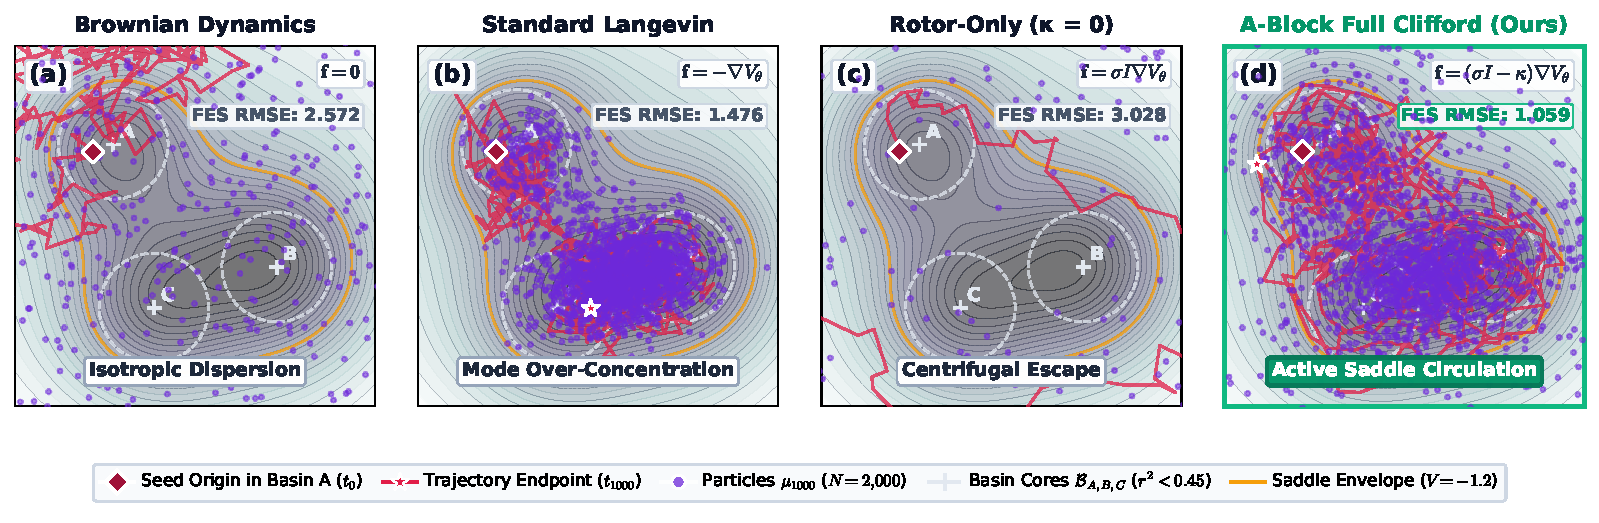
\includegraphics[width=\linewidth]{annotated_kinetic_trap_benchmark_1x4.pdf}
\vspace{-3mm}
\caption{Kinetic trap escape benchmark ($N=2{,}000$, $T=1{,}000$) initialized in Basin A, showing dashed basin core boundaries $\mathcal{B}_{A,B,C}$ ($r^2<0.45$) and the gold low-energy saddle envelope ($V=-1.2\text{ kcal/mol}$). (a)~Brownian dynamics exhibits undirected diffusion. (b)~Standard Langevin ($\kappa=1$) over-concentrates in basin cores due to uncalibrated score temperature. (c)~Rotor-only ($\kappa=0$) produces centrifugally divergent orbits. (d)~A-Block Full Clifford couples calibrated dilation with active saddle circulation, achieving the lowest FES RMSE ($1.059\text{ kcal/mol}$) and highest inter-basin transition frequency ($22.48$ transitions/particle).}
\label{fig:kinetic_trap_benchmark}
\vspace{-2mm}
\end{figure}

\subsection{Analysis of Benchmark Results, Ablations, and Sensitivity Checks}

\textbf{Isolating Contraction ($\kappa$) vs.\ Rotor Circulation ($\sigma I$).} Table~\ref{tab:moml_benchmarks} resolves the exact contribution of each operator. First, comparing Standard Langevin ($\kappa=1, \sigma=0$, $\text{RMSE} = 1.476\text{ kcal/mol}$) against Dilator-Only ($\sigma=0, \kappa$, $\text{RMSE} = 1.064\text{ kcal/mol}$) confirms Proposition~\ref{prop:stationarity}: because the dimensionless DSM potential $V_\theta$ scales as $\alpha_E \approx 1.68\text{ (kcal/mol)}^{-1}$, setting $\kappa=1$ over-concentrates particles inside the core radii $\mathcal{B}_B \cup \mathcal{B}_C$ ($60.9\%$ occupancy and low global transport distance $\mathcal{W}_1 = 0.066$) while under-sampling basin skirts and transition saddles (raising FES RMSE to $1.476$). Reducing contraction to $\bar{\kappa} \approx 0.33$ restores the Boltzmann temperature scale inside the wells ($\text{RMSE} = 1.064$), but at the cost of sluggish kinetics: Dilator-Only suffers a $35.4\%$ drop in inter-basin transition rate ($13.86$ transitions/particle) and incomplete trajectory visitation ($96.9\%$). Adding the Clifford rotor in \textbf{A-Block Full Clifford} preserves and improves the FES reconstruction accuracy ($\mathbf{1.059 \pm 0.031\text{ kcal/mol}}$, lowest variance across seeds) while boosting the inter-basin transition rate by $\mathbf{+62.2\%}$ ($22.48$ vs.\ $13.86$ transitions/particle) and restoring $99.7\%$ cumulative visitation. Meanwhile, A-Block's lower instantaneous terminal B/C core occupancy ($37.4\%$) reflects active steady-state circulation across the intermediate saddle pathways connecting all three basins ($V < -1.2$).

\textbf{Timestep ($dt$) and Histogram Bin Sensitivity.} Because explicit Euler integration of rotational drift $\sigma I \nabla V_\theta$ introduces $O(dt^2)$ radial truncation error (manifesting when $\kappa=0$ in Figure~\ref{fig:kinetic_trap_benchmark}c), we verified our benchmark at a $3\times$ smaller timestep ($dt = 0.005, T = 3{,}000$, identical physical horizon $T\cdot dt = 15.0$). At $dt = 0.005$, A-Block Full Clifford improves further ($\text{FES RMSE} = \mathbf{1.041\text{ kcal/mol}}$, $\mathcal{W}_1 = 0.316$, Terminal B/C Occupancy $= 41.4\%$, Cumulative Visitation $= \mathbf{99.9\%}$, and $\mathbf{25.99}$ transitions/particle vs.\ $1.503\text{ kcal/mol}$ for Standard Langevin and $16.14$ transitions/particle for Dilator-Only). Similarly, across histogram resolutions of $25\times 25$, $35\times 35$, and $50\times 50$ bins, A-Block consistently outperforms Standard Langevin ($0.809 / 1.059 / 1.287\text{ kcal/mol}$ vs.\ $1.298 / 1.476 / 1.549\text{ kcal/mol}$).

\section{Conclusion and Limitations}
We introduced \textit{A-Block}, a Clifford Neural Score Matching framework uniting $\operatorname{Cl}(2,0)$ rotor-dilator algebra with score-based SDEs and active particle hydrodynamics. Our theoretical and empirical analyses establish that pairing calibrated dilation with transverse bivector circulation simultaneously improves local free-energy reconstruction and accelerates inter-basin transitions. As a workshop contribution, our empirical validation is currently limited to 2D synthetic multi-well potentials and non-convex topological attractors (Appendix~\ref{sec:appendix}), and our $(\sigma, \kappa)$ operators act in a quasi-constant regime rather than via a supervised control objective. Future work will extend direct-sum dihedral rotors $\bigoplus_{k=1}^K \operatorname{Cl}(2,0)$ to coupled all-atom peptide backbones (e.g., alanine dipeptide and fast-folding miniproteins) and introduce variational path-space objectives to jointly supervise position-dependent rotor schedules.

\clearpage
\footnotesize
\bibliographystyle{unsrtnat}
\bibliography{reference}


\clearpage
\appendix
\section{Modular Multiscale Assemblies and Standardized Typography Benchmark}
\label{sec:appendix}

\begin{figure}[!htb]
\centering
\vspace{-2mm}
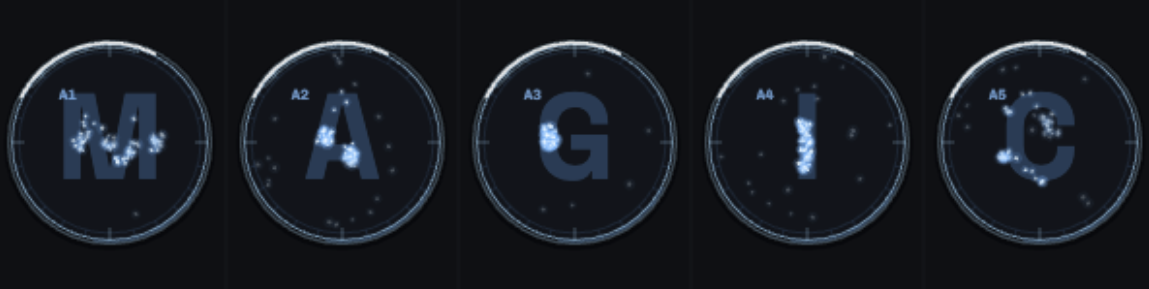
\includegraphics[width=0.73\linewidth]{d.png}
\vspace{-2mm}
\caption{Multi-unit A-Block ensemble ($A_1$--$A_5$) simulating active particle density measures $\mu_t$ under learned score fields $V_\theta(\mathbf{x})$ across target morphological attractors (\textit{``MAGIC''}). Non-convex letterforms serve as a 2D topological stress test for steric trapping: navigating the sharp inner spur of the letter \textit{`G'} without boundary arrest requires transverse rotor circulation ($\sigma I$) coupled with dilator confinement ($-\kappa$). Evaluating $K=5$ decoupled apertures in parallel empirically illustrates linear $\sum_k O(N_k) = O(N_{\text{total}})$ scaling without $O(N^2)$ pairwise proximity graphs.}
\label{fig:ablock_units}
\vspace{-2mm}
\end{figure}

In this Appendix, we illustrate the non-equilibrium active matter regime of A-Block (Proposition~\ref{prop:stationarity}, Case 2). An ensemble of $K=5$ parallel A-Block apertures ($A_1$--$A_5$, Figure~\ref{fig:ablock_units}) maintains independent empirical density measures $\mu_t = \frac{1}{N_k} \sum_{i=1}^{N_k} \delta_{\mathbf{x}_i(t)}$, eliminating quadratic $O(N^2)$ neighbor-graph overhead.

\subsection{Standardized Topological Navigation Benchmark on Non-Convex Glyphs}
To evaluate active spatial confinement and steric escape in non-convex geometries, we benchmarked all four dynamics on the upright letterform \textit{`G'} ($400\times 400$ grid, Figure~\ref{fig:typography_benchmark}). The potential $V(\mathbf{x}) = -\ln(G_{\sigma_b} * \mathbf{1}_{\text{glyph}}(\mathbf{x}) + 10^{-3}) + 0.08 \max(0, \|\mathbf{x}-\mathbf{c}\| - r_{\text{dish}})^2$ is constructed from the Gaussian-smoothed glyph mask ($\sigma_b = 7.5\text{ px}$). To ensure a strictly fair comparison, all four methods use the exact same initial seed in the sharp inner spur of the \textit{`G'} ($N=1{,}200$ particles, $T=4{,}000$ steps, $dt=2.0$), the exact same stochastic noise amplitude ($\text{noise\_amp}=0.85$), and identical circular aperture boundary clamping at $r_{\text{dish}} = 176\text{ px}$.

We report three complementary metrics in Figure~\ref{fig:typography_benchmark} and \texttt{output/typography\_metrics.json}: (1)~\textbf{In-Glyph Precision (\%):} percentage of particles residing strictly inside the binary glyph stroke mask at $t = T$; (2)~\textbf{Cumulative Trajectory Visitation (\%):} percentage of glyph pixels visited by the exact particle trajectories ($r = 0\text{ px}$ point coordinates) over $t \in [0, T]$; and (3)~\textbf{Terminal Steady-State Coverage (\%):} percentage of the glyph stroke covered by the final particle ensemble ($r = 8\text{ px}$ kernel footprint) at $t = T$.

\begin{figure}[!htb]
\centering
\vspace{-2mm}
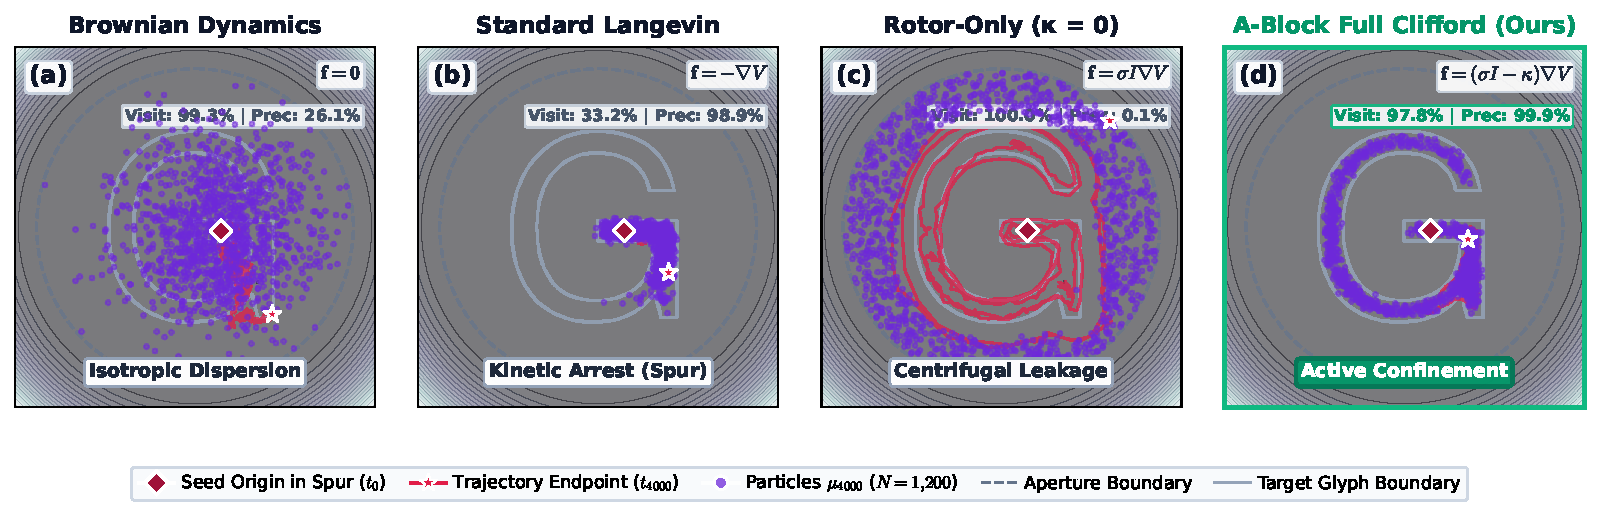
\includegraphics[width=0.84\linewidth]{typography_kinetic_trap_benchmark_1x4.pdf}
\vspace{-2mm}
\caption{Standardized topological navigation benchmark on the non-convex letterform \textit{`G'} ($N=1{,}200$, $T=4{,}000$, identical noise amplitude $0.85$ and circular aperture boundary $r_{\text{dish}}$ across all baselines). (a)~\textbf{Brownian Dynamics ($\mathbf{f}=\mathbf{0}$)}: Unbounded isotropic diffusion visits $99.3\%$ of the glyph over time ($90.5\%$ terminal coverage) but leaks indiscriminately into the surrounding void (\textbf{Precision: $26.1\%$}). (b)~\textbf{Standard Langevin ($\sigma=0, \kappa=1.0$)}: Pure inward gradient drift confines particles to the stroke (\textbf{Precision: $98.9\%$}) but suffers severe kinetic arrest in the initial inner spur pocket (\textbf{Trajectory Visitation: $33.2\%$}, \textbf{Terminal Coverage: $33.7\%$}). (c)~\textbf{Rotor-Only ($\sigma=11.0, \kappa=0$)}: Transverse circulation sweeps across the domain (\textbf{Visitation: $100.0\%$}) but centrifugal drift flings particles to the outer aperture wall (\textbf{Precision: $0.1\%$}, \textbf{Terminal Coverage: $1.4\%$}). (d)~\textbf{Full Clifford A-Block ($\sigma=11.0, \kappa=1.8$)}: Coupled rotor-dilator dynamics propel particles tangentially around the $180^\circ$ bends while clamping them inside the stroke, achieving \textbf{$99.9\%$ In-Glyph Precision}, \textbf{$97.8\%$ Cumulative Trajectory Visitation}, and \textbf{$99.2\%$ Terminal Coverage}.}
\label{fig:typography_benchmark}
\vspace{-2mm}
\end{figure}

Because $-\nabla V(\mathbf{x})$ points perpendicularly inward toward the medial axis of the letter stroke, pure gradient descent (Standard Langevin, $\sigma=0, \kappa=1.0$, and matched Dilator-Only, $\sigma=0, \kappa=1.8$, which reaches $31.2\%$ visitation and $33.6\%$ terminal coverage) generates zero tangential propulsion along the contour, leaving $>66\%$ of the glyph unvisited. Conversely, Rotor-Only ($\kappa=0$) suffers complete centrifugal escape to the dish rim. A-Block's rotor-dilator flow $(\sigma I - \kappa)\nabla V$ converts dead-end steric corners into continuous circulation channels while maintaining $99.9\%$ spatial confinement.

\end{document}
